%%%%%%%%%%%%%%%%%%%%%%%%%%%%%%%%%%%%%%%%%
% University Assignment Title Page 
% LaTeX Template
% Version 2.0 (21/04/18)
% Modified by
% Erdem TUNA &
% Halil TEMURTAŞ
%
% This template has been downloaded from:
% http://www.LaTeXTemplates.com
%
% Original author:

% Instructions for using this template:
% This title page is capable of being compiled as is. This is not useful for 
% including it in another document. To do this, you have two options: 
%
% 1) Copy/paste everything between \begin{document} and \end{document} 
% starting at \begin{titlepage} and paste this into another LaTeX file where you 
% want your title page.
% OR
% 2) Remove everything outside the \begin{titlepage} and \end{titlepage} and 
% move this file to the same directory as the LaTeX file you wish to add it to. 
% Then add \input{./title_page_1.tex} to your LaTeX file where you want your
% title page.
%
%%%%%%%%%%%%%%%%%%%%%%%%%%%%%%%%%%%%%%%%%
%\title{Title page with logo}
%----------------------------------------------------------------------------------------
%	PACKAGES AND OTHER DOCUMENT CONFIGURATIONS
%----------------------------------------------------------------------------------------

\documentclass[12pt]{article}
\usepackage[english]{babel}
\usepackage[utf8x]{inputenc}
\usepackage{amsmath}
\usepackage{graphicx}
\usepackage[colorinlistoftodos]{todonotes}
\usepackage{gensymb} % this could be problem
\usepackage{float}
\usepackage{fancyref}
\usepackage{subcaption}
\usepackage[toc,page]{appendix} %appendix package
\usepackage{xcolor}
\usepackage{listings}
\usepackage{xspace}


\usepackage{amssymb}
\usepackage{nicefrac}
\usepackage{gensymb}
\usepackage{xspace}
\usepackage{fancyhdr}





\newcommand\nd{\textsuperscript{nd}\xspace}
\newcommand\rd{\textsuperscript{rd}\xspace}
\newcommand\nth{\textsuperscript{th}\xspace} %\th is taken already


\definecolor{mGreen}{rgb}{0,0.6,0} % for python
\definecolor{mGray}{rgb}{0.5,0.5,0.5}
\definecolor{mPurple}{rgb}{0.58,0,0.82}
\definecolor{mygreen}{RGB}{28,172,0} % color values Red, Green, Blue for matlab
\definecolor{mylilas}{RGB}{170,55,241}





\lstdefinestyle{CStyle}{
    commentstyle=\color{mGreen},
    keywordstyle=\color{magenta},
    numberstyle=\tiny\color{mGray},
    stringstyle=\color{mPurple},
    basicstyle=\footnotesize,
    breakatwhitespace=false,         
    breaklines=true,
    frame=single,
    rulecolor=\color{black!40},                 
    captionpos=b,                    
    keepspaces=true,                 
    numbers=left,                    
    numbersep=5pt,                  
    showspaces=false,                
    showstringspaces=false,
    showtabs=false,                  
    tabsize=2,
    language=C
}


\lstset{language=Matlab,%
    %basicstyle=\color{red},
    breaklines=true,%
    frame=single,
    rulecolor=\color{black!40},
    morekeywords={matlab2tikz},
    keywordstyle=\color{blue},%
    morekeywords=[2]{1}, keywordstyle=[2]{\color{black}},
    identifierstyle=\color{black},%
    stringstyle=\color{mylilas},
    commentstyle=\color{mygreen},%
    showstringspaces=false,%without this there will be a symbol in the places where there is a space
    numbers=left,%
    numberstyle={\tiny \color{black}},% size of the numbers
    numbersep=9pt, % this defines how far the numbers are from the text
    emph=[1]{for,end,break},emphstyle=[1]\color{red}, %some words to emphasise
    %emph=[2]{word1,word2}, emphstyle=[2]{style},    
}



\makeatletter
\renewcommand\paragraph{\@startsection{paragraph}{4}{\z@}%
            {-2.5ex\@plus -1ex \@minus -.25ex}%
            {1.25ex \@plus .25ex}%
            {\normalfont\normalsize\bfseries}}
\makeatother
\setcounter{secnumdepth}{4} % how many sectioning levels to assign numbers to
\setcounter{tocdepth}{4}    % how many sectioning levels to show in ToC



% For Blank Page -------------
\newcommand{\blankpage}{
	\- \\[8.5cm]	
	{ \centering This Page Intentionally Left Blank \par }
	\- \\[8.5cm]
}
% ---------------------------

%\begin{figure}[H]
%	\setlength{\unitlength}{\textwidth} 
%	\centering
%	\begin{subfigure}{.5\textwidth}
%  		\centering
%  		\includegraphics[width=0.48\unitlength]{SubFigure1}
%  		\caption{\label{fig:As12}SubFigure2 }
%	\end{subfigure}%
%	\begin{subfigure}{.5\textwidth}
%  		\centering
%		\includegraphics[width=0.48\unitlength]{SubFigure2}
%  		\caption{\label{fig:As12}SubFigure2 }
%	\end{subfigure}
%\caption{\label{fig:As12}Figure }
%\end{figure}



\begin{document}

\begin{titlepage}

\newcommand{\HRule}{\rule{\linewidth}{0.5mm}} % Defines a new command for the horizontal lines, change thickness here

\center % Center everything on the page
%----------------------------------------------------------------------------------------
%	LOGO SECTION
%----------------------------------------------------------------------------------------


\includegraphics[scale=0.3]{odtuee.png}\\[1cm]
% Include a department/university logo - this will require the graphicx package
 
%----------------------------------------------------------------------------------------

 
%----------------------------------------------------------------------------------------
%	HEADING SECTIONS
%----------------------------------------------------------------------------------------

\textsc{\LARGE Middle East Technical University}\\[1.5cm] % Name of your university/college
\textsc{\Large Department of Electrical and Electronics Engineering }\\[0.5cm] % Major heading such as course name
 % Minor heading such as course title

%----------------------------------------------------------------------------------------
%	TITLE SECTION
%----------------------------------------------------------------------------------------

\HRule \\[0.4cm]

{ \huge \bfseries \large EE400 Summer Practice II \\ Report}\\[0cm] % Title of your document
\HRule \\[1cm]
 
%----------------------------------------------------------------------------------------
%	AUTHOR SECTION
%----------------------------------------------------------------------------------------

\begin{minipage}{0.38\textwidth}
\begin{flushleft} \large
	\textbf{Student Name:} \\
		\textit{Halil Temurtaş} \\
	\textbf{Student ID:} \\ 
		\textit{2094522} \\
	\textbf{SP Beginning Date:} \\
		\textit{09.07.2018} \\
	\textbf{SP End Date:}\\
		\textit{03.08.2018} \\
	\textbf{EE300 SP Location:} \\ 
		\textit{TÜRKSAT A.Ş.} 
\end{flushleft}
\end{minipage}
\begin{minipage}{0.6\textwidth}
\begin{flushright} \large
	\textbf{EE400 SP Company Name:} \\ 
		\textit{ASELSAN A.Ş.} \\
	\textbf{EE400 SP Company Division:} \\ 
		\textit{HBT Test ve Süreç Tasarımı Mdl.} \\
	\textbf{Supervisor Engineer:} \\
		\textit{Pınar Kırıkkanat} \\
	\textbf{SE Contact Mail:} \\
		\textit{pkirikkanat@aselsan.com.tr}  \\
	\textbf{SE Contact Phone:} \\
		\textit{+90 (312) 592 19 17 } 
\end{flushright}
\end{minipage}\\[0.8cm]

% If you don't want a supervisor, uncomment the two lines below and remove the section above
%\Large \emph{Author:}\\
%John \textsc{Smith}\\[3cm] % Your name

%----------------------------------------------------------------------------------------
%	DATE SECTION
%----------------------------------------------------------------------------------------

{\large 21/08/2018}\\[1cm] % Date, change the \today to a set date if you want to be precise


\vfill % Fill the rest of the page with whitespace

\end{titlepage}


\blankpage



\tableofcontents
\newpage


%\begin{abstract}
%Your abstract.
%\end{abstract}

\section{Introduction}
\-\indent 
	I performed my summer practice in ASELSAN A.Ş., one of leading defence industry companies in Turkey. my internship lasted 20 days and Pınar Kırıkkanat, an electronics engineer in ASELSAN was my supervisor and assisted me in my summer practice.

	The summer practice started with an orientation program that briefly explains the company and how the works are handled. Following that, mandatory educations like occupational safety and health education is given to the interns by the company. After the educations, inters were sent to their assigned departments and division. I was similarly sent to HBT division to perform my summer practice.
	
	In the first half of my internship, I was given time to observe, learn and participate the mechanical and electrical test conducted at our division. Mainly on ASELSAN 9661 Series Radios, I mostly observed and participated on the environmental tests of the equipments produced at the Communication \& Information Technologies Vice Presidency, known as HBT. .
	
	In the second part of my internship, I was given time to observe the work done behind the testing, in other words process design and management. In this part of my internship, I participated on documentation and research activities for the ULAK Base station of the ASELSAN. Since the work done at this stage can be mostly considered as classified information, I will mention the basics of what I have done in this part.
	
	In this, report, I start with an introduction, that covers what was done in my summer practice. Then, I continued with a company description section in which the general description about ASELSAN is given. After that part, the work done in my summer practice is explained. Lastly, I finished the report with an conclusion part. 
	
	
%\- \\[2cm]
 

\section{Description of the Company}
\- \indent
	In this chapter, I will introduce the company in five main parts:



\subsection{Company Name}
\-
\indent ASELSAN A.Ş. or \textbf{AS}KERİ \textbf{EL}EKTRONİK \textbf{SAN}AYİ A.Ş.


\subsection{Company Locations}
\-\indent
	ASELSAN has six campuses in Turkey, one of them being in Istanbul, other campuses are located at Ankara. Throughout my summer practice, I spent my time at \textbf{Macunköy} Facilities . 
\\
\\
\textbf{ Address / Macunköy Facilities:} Mehmet Akif Ersoy Mahallesi 296. Cadde No: 16, 06370 Yenimahalle-Ankara, Türkiye
\\
\\
\textbf{ Phone:} +90 (312) 592 10 00
\\
\\
\textbf{ Fax:} +90 (312) 354 13 02 / +90 (312) 354 26 69


\subsubsection{Macunköy Facilities}
\- \indent

	Macunköy Facilities was established on an area of total 186.000 m2, 110.000 m2 of which is the closed area. \textbf{General Directorate}, \textbf{SST} Group, \textbf{UGES} Group and parts of \textbf{HBT} and \textbf{REHİS} Groups are at Aselsan Macunköy Facilities.



\subsubsection{Other Facilities}


\begin{itemize}
\item Akyurt Facilities (\textbf{MGEO} Group)
\item Gölbaşı Facilities (\textbf{REHİS} Group)
\item ODTÜ TEKNOKENT (SATGEB Building) (Part of \textbf{HBT} Group)
\item ODTÜ TEKNOKENT (TİTANYUM Building) (Part of \textbf{HBT} Group)
\item İstanbul Facilities (Part of \textbf{SST} Group)
\end{itemize}



%\vfill

\subsection{General Description of the Company}
\-
\indent ASELSAN is a company of Turkish Armed Forces Foundation, established in 1975 after Cyprus Peace Operation in order to meet the communication needs of the Turkish Armed Forces by national means. Currently 74,20\% of the shares are owned by the Foundation whereas the remaining 25,70\% runs in İstanbul Borsa stock market.

	As one of the largest defence industry companies of Turkey, ASELSAN's product portfolio includes communication and information technologies, radar and electronic warfare, electro-optics, avionics, unmanned systems, land, naval and weapon systems, air defence and missile systems, command and control systems, transportation, security, traffic, automation and medical systems as can be seen from the  \textit{Figure~\ref{fig:As12}}. 
	
%	Today ASELSAN has become an indigenous products exporting company, investing in international markets through various cooperation models with local partners and listed as one of the top 100 defence companies of the world (Defense News Top 100).

\begin{figure}[H]
\center
\setlength{\unitlength}{\textwidth} 
%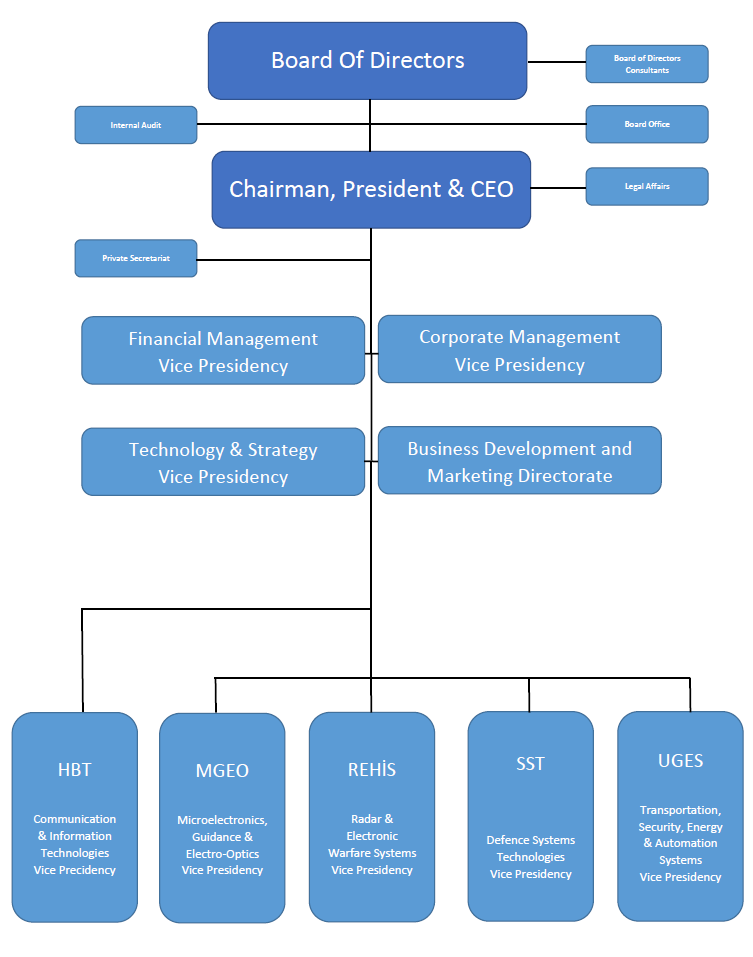
\includegraphics[width=0.9\unitlength]{organizasyon2}
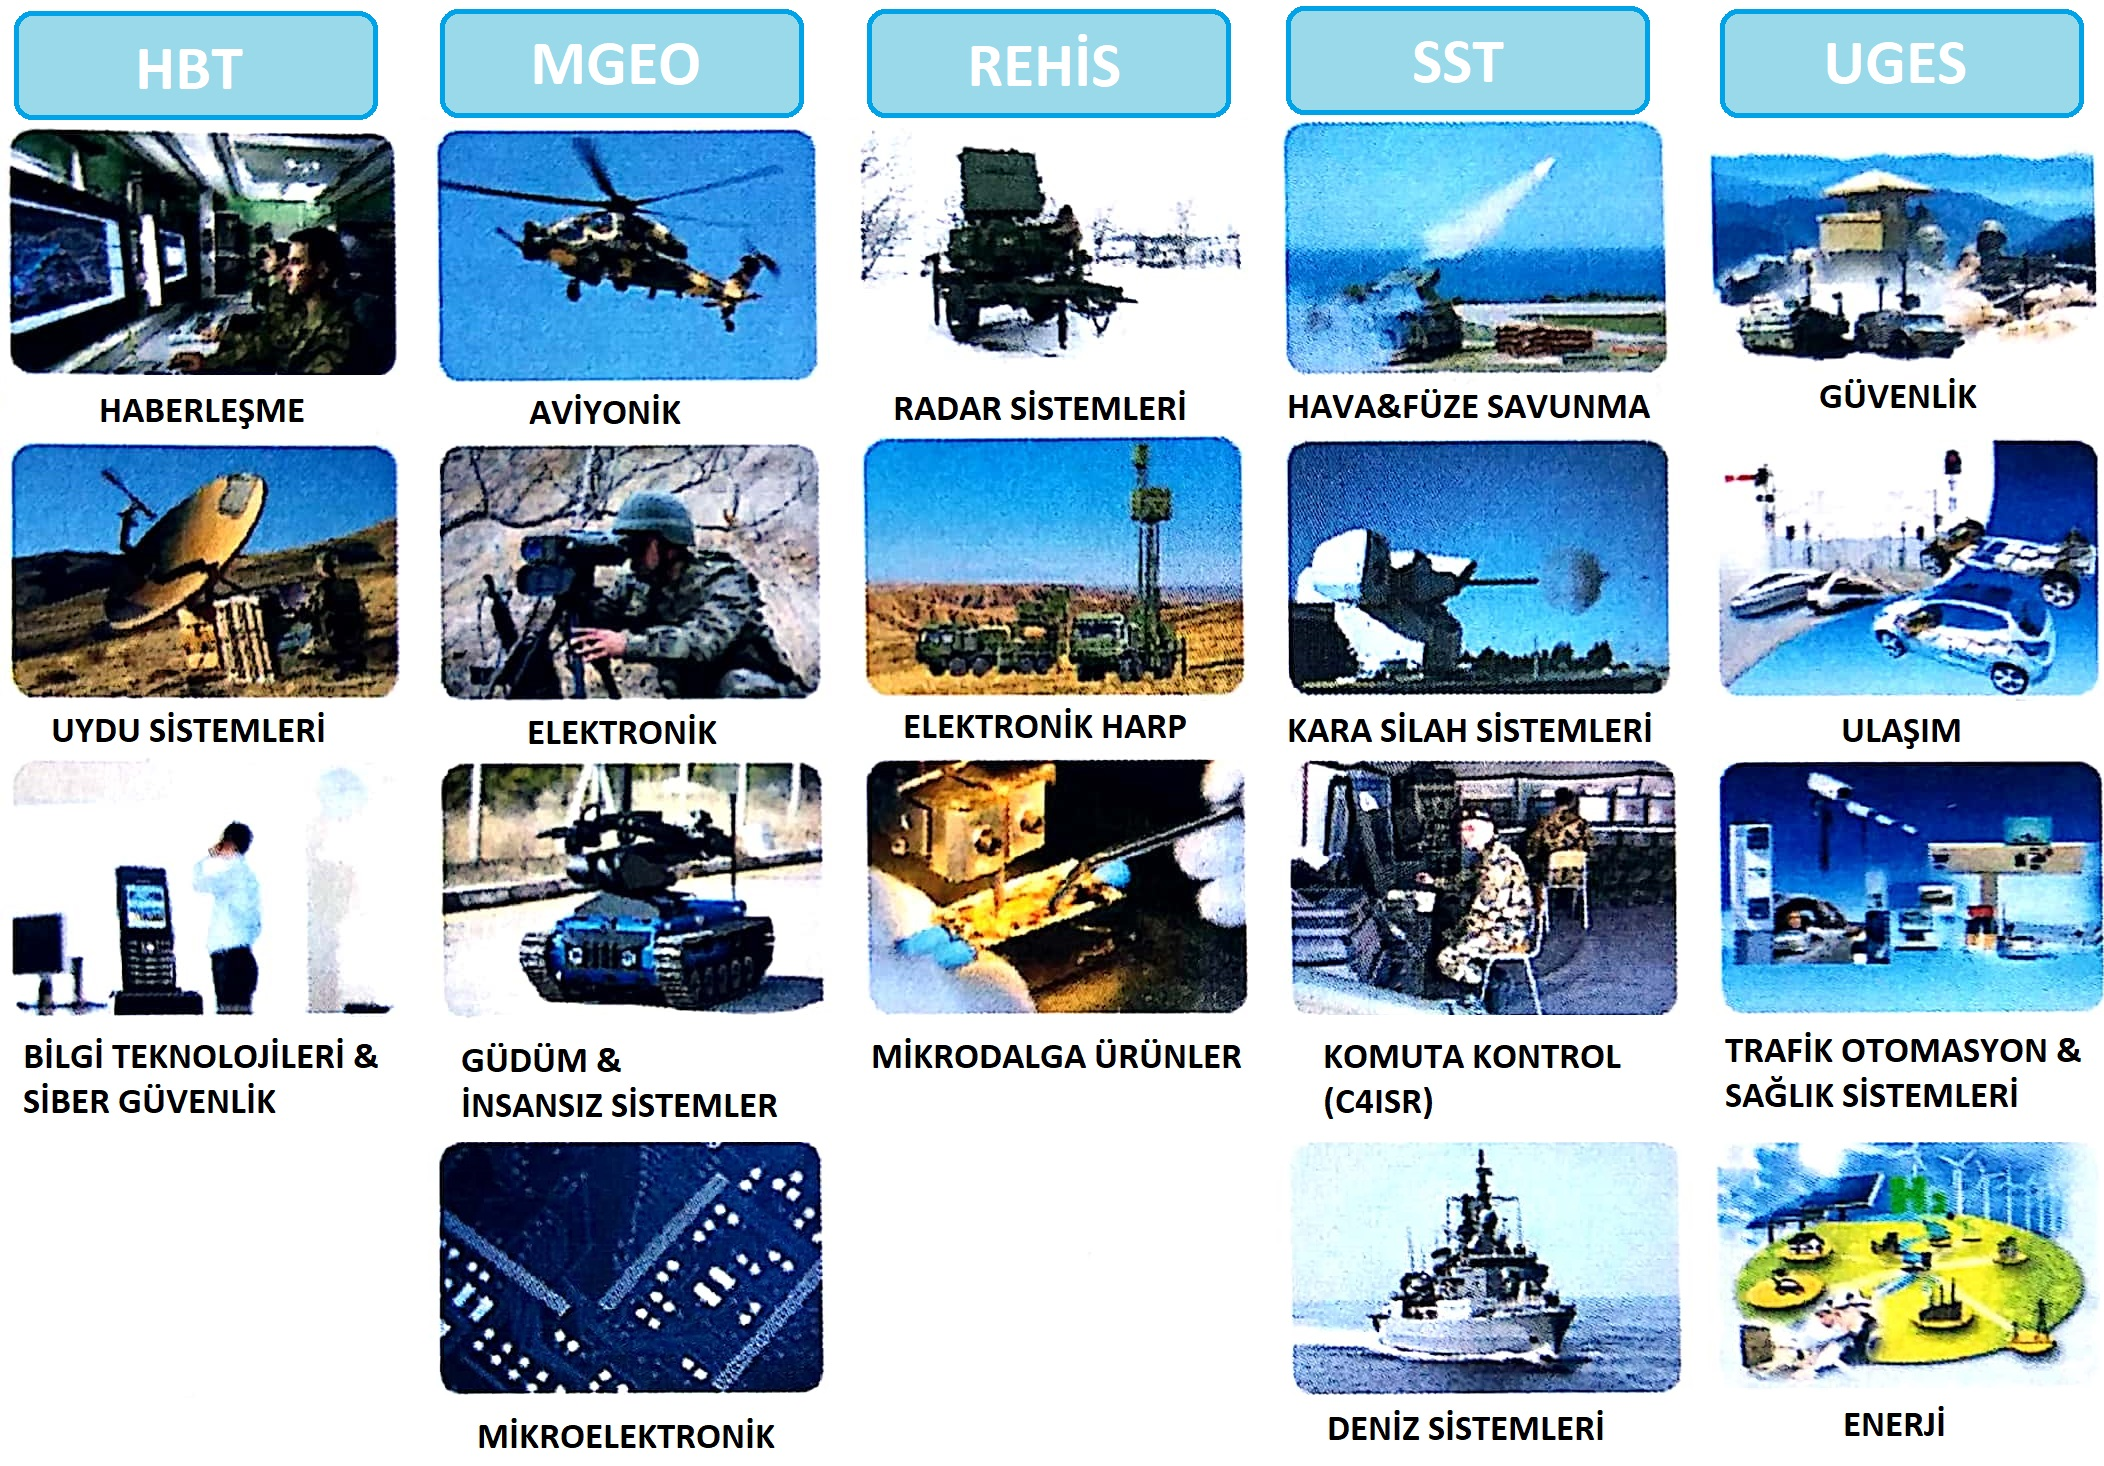
\includegraphics[width=0.7\unitlength]{Aselsan1_2}
\caption{\label{fig:As12}Business Fields of ASELSAN }
\end{figure}

%	ASELSAN, together with the technology emphasis in its vision, has targeted to be a company that maintains its sustainable growth by creating value in the global market; preferred due to its competitiveness, trusted as a strategic partner, and caring for the environment and people.

	In 2018, ASELSAN is listed as 55\nth biggest defense company worldwide in DefenseNews' Top 100 list\cite{defense}. And as of July 2018, ASELSAN has 5364 employees. 63\% of them being engineer exact distribution of the employees can be seen at \textit{Figure~\ref{fig:calisan}}, while the academic distribution of the working engineers can be seen at \textit{Figure~\ref{fig:degree}}.

%	Together with the highly qualified engineering staff within more than 5000 employees, being the main driving factor of the company's success, ASELSAN allocates 6\% of its annual income for self-financed research and development activities.




\begin{figure}[H]
	\setlength{\unitlength}{\textwidth} 
	\centering
	\begin{subfigure}{.5\textwidth}
  		\centering
  		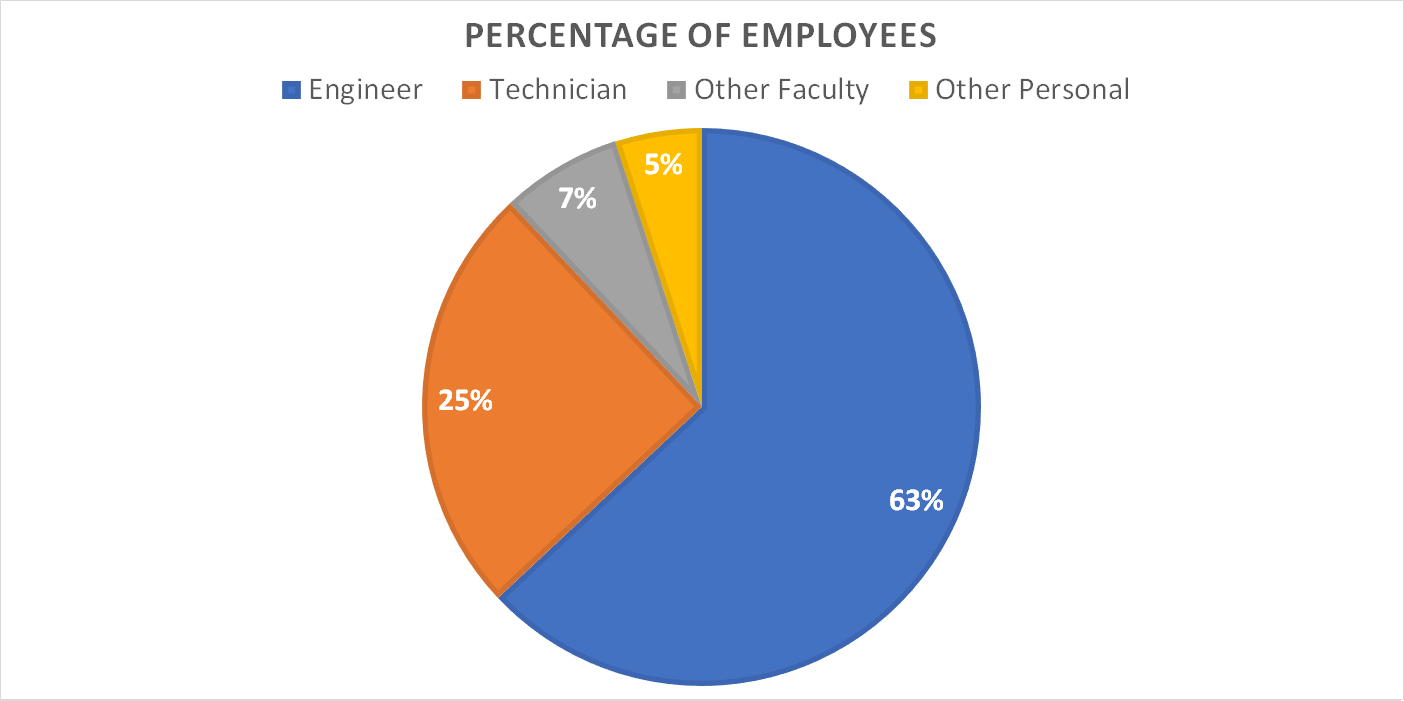
\includegraphics[width=0.48\unitlength]{calisan}
  		\caption{\label{fig:calisan}Distribution of the Employees }
	\end{subfigure}%
	\begin{subfigure}{.5\textwidth}
  		\centering
		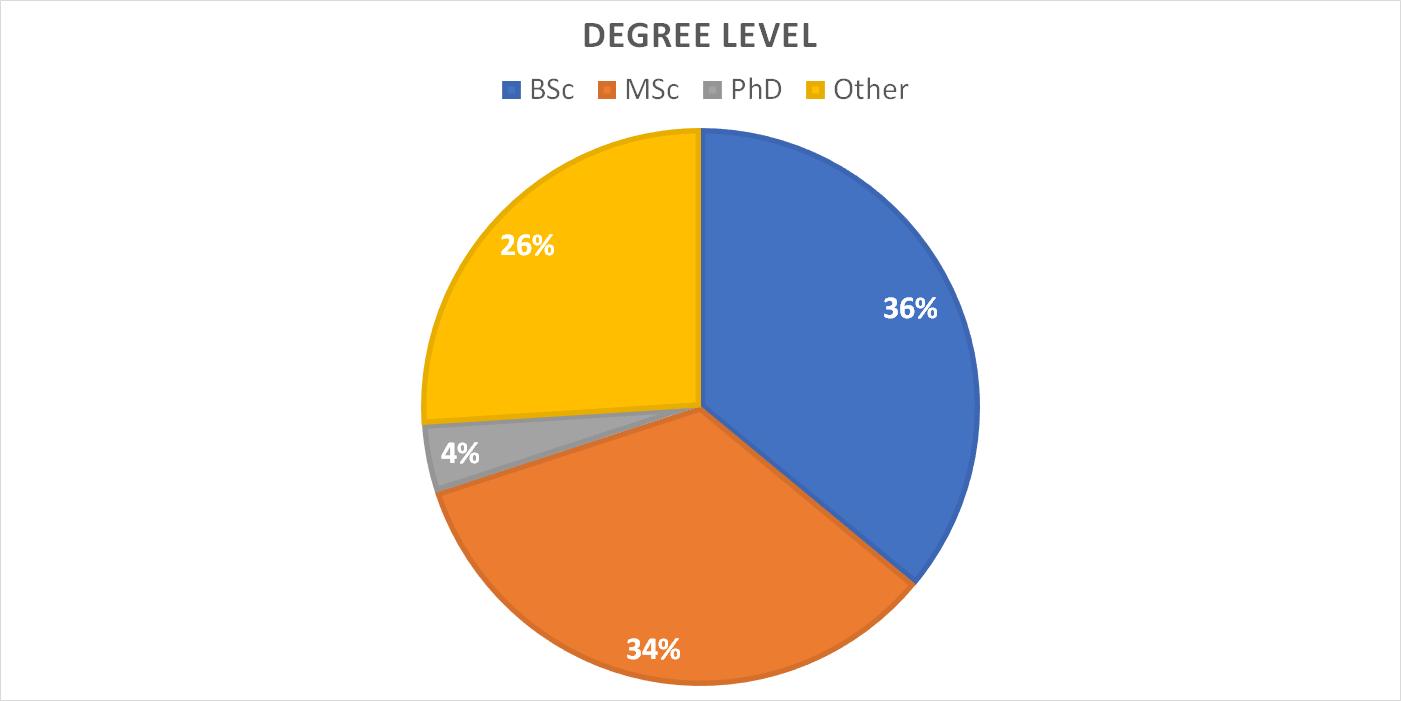
\includegraphics[width=0.48\unitlength]{degree}
  		\caption{\label{fig:degree}Degree Levels of the Engineers }
	\end{subfigure}
\caption{\label{fig:calisandegree} Statistics about ASELSAN Employees   }
\end{figure}


	
	
\vfill
\subsection{The Organizational Chart of the Company}
\-
\indent
The organizational chart of ASELSAN can be seen in \textit{Figure~\ref{fig:orgc}}.

\begin{figure}[H]
\center
\setlength{\unitlength}{\textwidth} 
%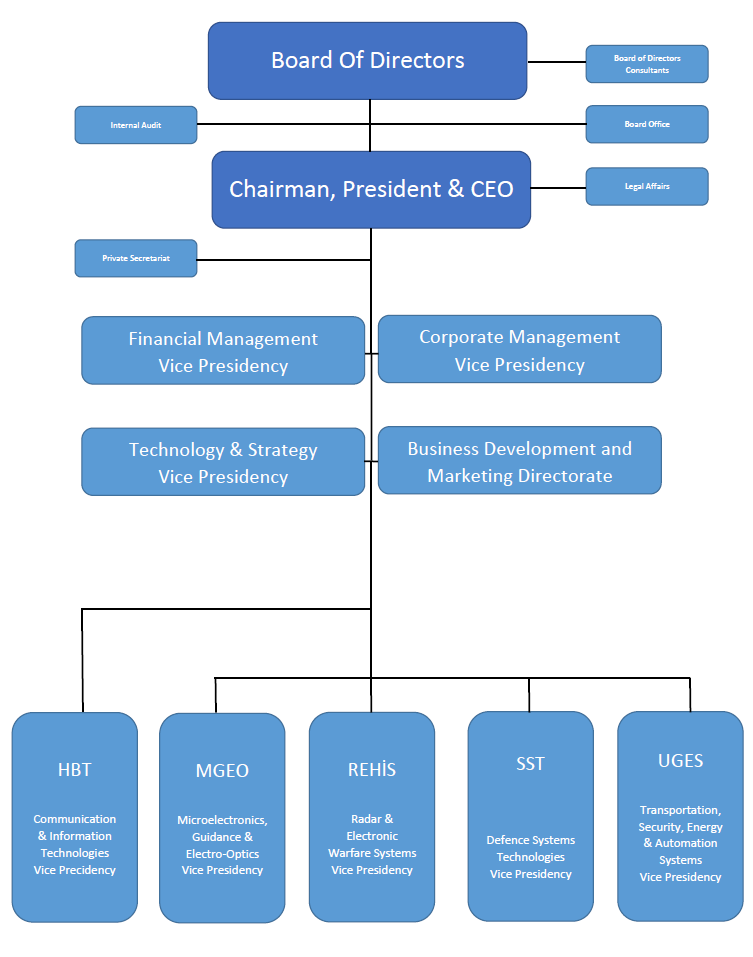
\includegraphics[width=0.9\unitlength]{organizasyon2}
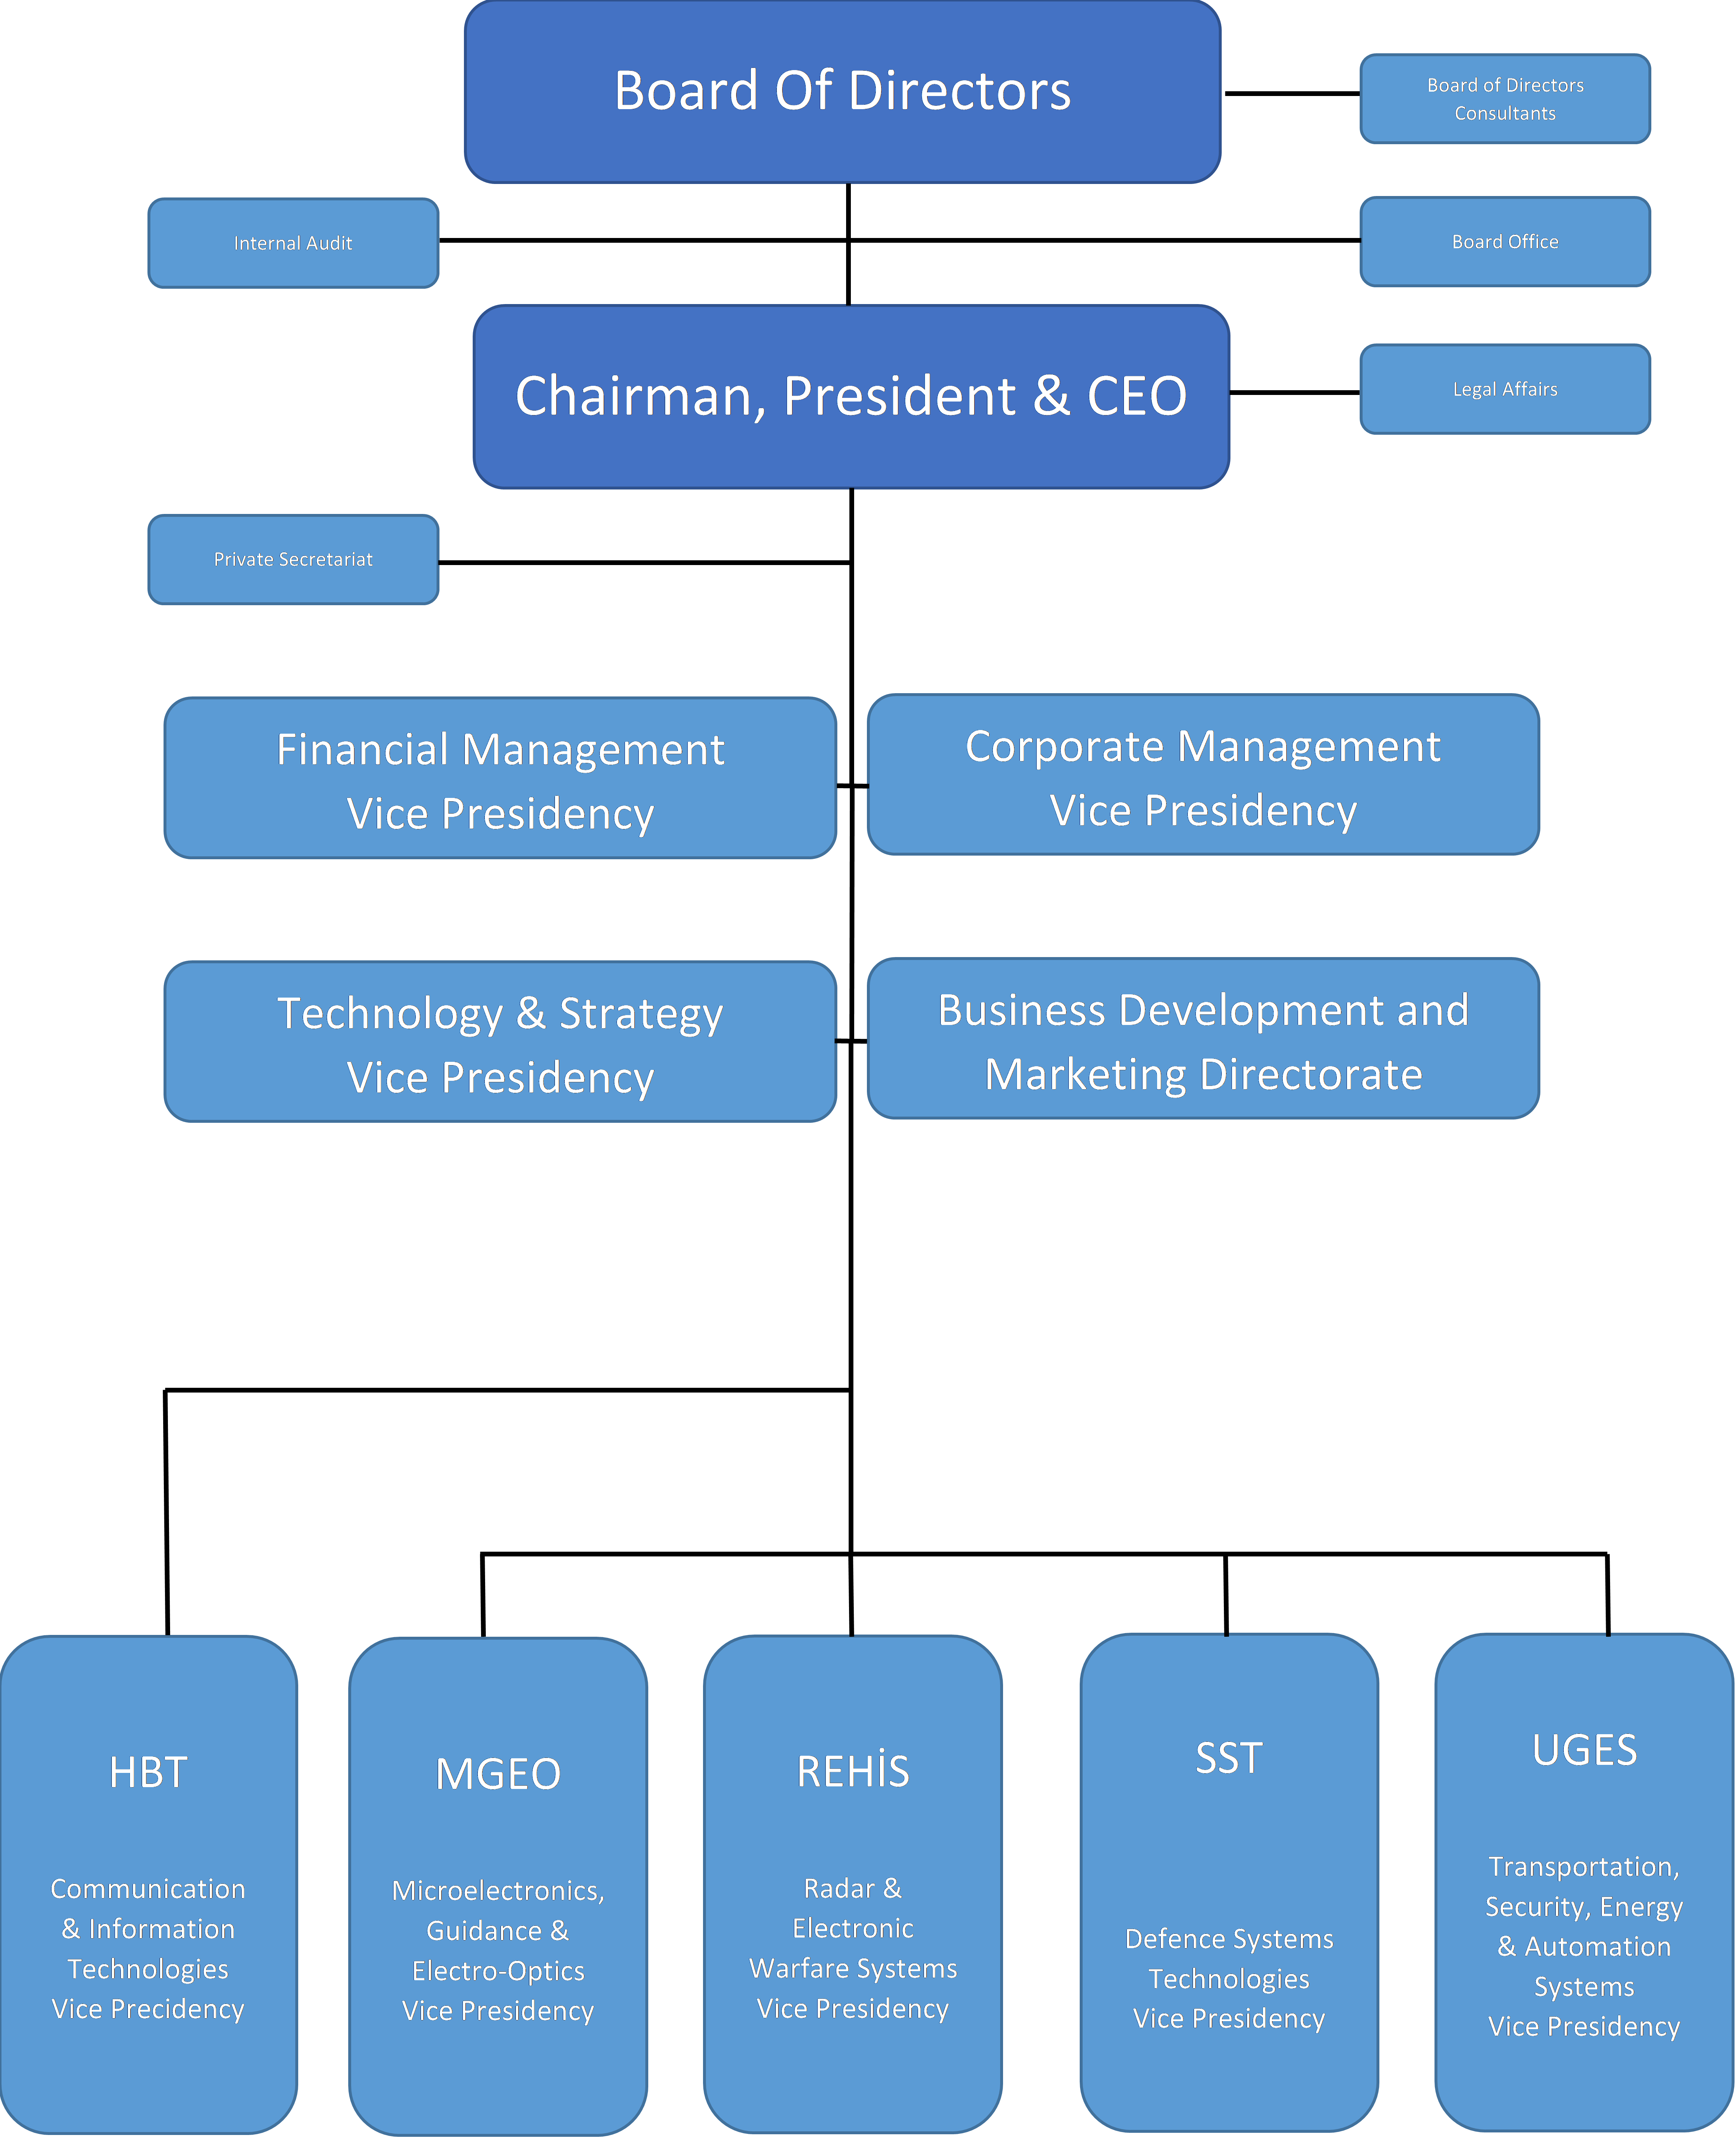
\includegraphics[width=0.93\unitlength]{organizasyon4}
\caption{\label{fig:orgc}The Organizational Chart of ASELSAN }
\end{figure}

		

\subsection{A Brief History of the Company}
\begin{itemize}
%\item \textbf{1976} 
%\subitem M. Hâcim KAMOY was assigned as the General Manager.
\item \textbf{ 1978 } : The first premises in Macunköy Facility were completed and the manufacturing operation started.
\item \textbf{ 1980 } : The first manpack and tank wireless radios were delivered to the Turkish Armed Forces.
%\item \textbf{ 1981 }
%\subitem The first hand-held radio and Bank Alarm Systems were designed. 
\item \textbf{ 1983 } : The first export was realized. 
\item \textbf{ 1982-1985 } : New products such as Field Telephones, Computer Controlled Central Systems and Laser Distance Measurement Appliances were included in the inventory. 
%\item \textbf{ 1986  }
%\subitem ASELSAN contributed to the power of Turkish Armed Forces with the Electronic Warfare and Data Terminal appliances it developed. 
\item \textbf{  1987 } : ASELSAN was included in a common project attended by 4 NATO countries for the manufacturing of Stinger Missile and started the required investment for the thick film hybrid circuit production. 
\item \textbf{  1988 } : ASELSAN produced the first avionic appliance for the F-16 program.
\item \textbf{ 1989 } : The first technology transfer to Pakistan was realized. Wireless radio production was started with ASELSAN license in NTRC facilities in Pakistan. 
\item \textbf{  1990 } : On date 21.05.1990, the ASELSAN shares were offered to the public and as of date 01.08.1990, the shares were started to be traded in IMKB (İstanbul Stock Exchange)
%\subitem ASELSAN was restructured in the 3 groups according to its fields of activity.
%\item \textbf{ 1991 }
%\subitem A Radar Technology Center was established in Aselsan with the SSIK 91-3 decision.
\item \textbf{ 1992 } : The Radar systems were included in the ASELSAN product range.
%\item \textbf{ 1992 }
%\subitem An Electro-Optical Technology Center was established in Aselsan with the SSIK 92-4 decision.
%\item \textbf{ 1994 }
%\subitem Studies with regard to design, assembly and commissioning works for Highway Emergency Assistance Communication Systems and Toll Collection Systems %and marketing of the same to foreign countries were started.
%\item \textbf{ 1995 }
%\subitem Project activities in main subjects such as Microelectronic, Guidance and Electro-Optical Group with the ongoing works and Hybrid Micro electronic, Inertial Navigational System, Infrared Guiding, Laser Guiding, Thermal Imaging Sensors, Passive Imaging Concentrators, Laser Generators and Sensors were realized.
%\item \textbf{ 1995 }
%\subitem Integration studies with regard to the applicability of electro-optical systems to different platforms and their more effective usage were realized and furthermore the production of ring laser gyroscope INS system was started.
\item \textbf{ 1996 } : The TASMUS agreement was executed.
\item \textbf{ 1997 } : ASELSAN 1919 Mobile Phone was launched to the market.
\item \textbf{ 1998 } : Thermal cameras, thermal weapon sight and thermal vision devices with target coordination addressing devices were submitted to the use of Turkish Armed Forces.
\item \textbf{ 1999 } : Agreements for Air Defence Early Warning and Command Control System, MILSIS Electronic Warfare and X-Band Satellite Communication System were executed.
%\item \textbf{ 2000 }
%\subitem Necip Kemal BERKMAN was assigned as the General Manager.
\item \textbf{ 2001 } : ASELSAN took over 72\% of the shares of ASELSAN MİKES A.Ş.
%\subitem The project for the serial production of KMS systems was executed. 
\item \textbf{ 2002 } : The equity capital of the company increased two and a half times compared to the previous year and reached the level of approximately one fourth of the aggregate resources.
%\subitem The Project for MWS-TU Missile Warning System and Leopard Volkan Fire Control System to be used in the Turkish Armed Forces Air Platforms was executed.
%\item \textbf{ 2003 }
%\subitem Agreements covering a long period for big projects such as SPEWS-II F-16 Electronic Warfare Auto Defense System, Military Police Integrated Communication and Information System were executed.
%\item \textbf{ 2004 }
%\subitem HEWS-CMDS CHAFF/FLARE shooter system Project was executed
\item \textbf{ 2005 } : HEWS, Helicopter Laser Warning Receiver system (LIAS) Project and Turkish Land Forces Avionic System Modernization Project was executed.
%\item \textbf{ 2006 }
%\subitem Cengiz ERGENEMAN was assigned to the General Manager position, Fuat AKÇAYÖZ was assigned as the Group President of Microwave and System Technologies, Dr. Faik EKEN was assigned as the Communication Devices Group President and KAHRAMANGİL was assigned as the Micro Electronic, Guidance and Electro-Optical Group President.
%\subitem ASELPOD Project was executed.
\item \textbf{ 2007 } : The construction of ASELSAN Integration Hall Building was completed and settlement activities were realized.
\item \textbf{ 2007 } : MILGEM war system supply project was executed.
\item \textbf{ 2008 } : ATAK agreement and Multi Band Digital Common Wireless Radio (ÇBSMT) Project were executed and ASELSAN delivered the first originally developed Air Defense Radar.
%\subitem In January 2008, Microwave and System Technologies Group Presidency was restructured as Defense System Technologies and Radar, Electronic Warfare and Communication Systems Group Presidency. Fuat AKÇAYÖZ was assigned to the position of Group President of Defense System Technologies and Ergun BORA was assigned to the position of Group President of Radar, Electronic Warfare and Communication Systems.
%\subitem In 2008, Coast Guard Command search and rescue Project, AKSAZ and FOCA Naval base under and surface surveillance and acquisition system (Yunus) Project, New Type Police Station Boat Project and JEMUS Kastamonu, Konya Wireless Radio system projects were executed. 
\item \textbf{ 2009 } : In 2009, four Research and Development Centrals were established, Leopard-1 Tank modernization was completed, MILGEM Warfare System 2nd Vessel Project, Ammunition Transfer system Project for Self-Propelled Howitzer (Fırtına- Storm) Ammunition vehicle and SAR / Reconnaissance System Supply Integration Project were executed.
%\subitem In 2009, STAMP and SOP system project for UAE, ADOP-2000 Fire Support System project, and the project for Land Located remote ED/ET capability gaining projects were executed.
%\item \textbf{ 2010 }
%\subitem In the year 2010, 112 Emergency Call Center was established in Antalya and Isparta, the Digital Trunk wireless radio system tender of İzmir Metropolitan Municipality was won and Tasmus-G 2nd Army Project deliveries were realized.
%\subitem In the year 2010, within the requirement by UAE, the subcontracting agreement was executed with Raytheon Company for the Patriot Missile System Antenna Mast Group products, ATMACA Electronic Systems development project, Pakistan Ministry of Defense Software Based Wireless Radio project, Naval Platform 3B Research Radar project, Self-propelled Air Defense Artillery and Fire Administration System Development project, 12 Air Defense Radar projects and 35 MM Towing Air Defense Artillery Modernization and Fragmentation Ammunition Development project were executed.
%\item \textbf{ 2011 }
%\subitem Following the manufacturing and plant acceptance tests of the Shipborne LPI Radar system ALPER (ASELSAN Low Power ECCM Radar) originally developed developed by ASELSAN, it was integrated to the TCG Heybeliada corvette within the scope of MILGEM Project, the Harbor Acceptance Tests were completed successfully and the first duty was started after the completion of the delivery.
%\subitem In the year 2011, MILGEM 1 Ship TCG HEYBELİADA Naval Acceptance Tests were completed successfully and was delivered to the navy. "AY Class Diesel-Electric Submarines Upgrade Project" was executed between . SSM, ASELSAN, STM and RAYTHEON companies. "Lower and Medium Altitude Air Defense Missile System Project Design and Development Period Agreement" was executed between SSM and ASELSAN. On date 12 April 2011, President Abdullah Gül visited the Macunköy Facility.
%\item \textbf{ 2012 }
%\subitem In May 2012 Necmettin BAYKUL was assigned as board of Directors. By the city hall, the name “Hacim KAMOY” founder of ASELSAN, has been given to the park nearby Macunköy facilities.
\item \textbf{  2012 } : Turkey’s first national Air Defense System “Pedestal Mounted Stinger System” which has been designed and produced by ASELSAN, and whose delivery took nearly 23 years, last 5 pieces has been delivered to Turkish Armed Forces.
\item \textbf{ 2013 } : ASELSAN has continued its climb for the aim of being one of the top 50 defense companies, and ranked 74th according to annual sales.
\item \textbf{ 2013 } : ASELSAN was the company who has participiated most at the 11th International Defence Industry Fair (IDEF 2013).	
%\subitem ASELSAN has won the “Leadership at Technology” award at the inovation week organized by Turkish Exporters’ Association. ASELSAN has also won “ Year 2013 Innovativeness Creativity Product Award”among the large companies with the SERHAT Counter Mortar Radar product at the event of TESİD Innovativeness Creativity Awards.

\end{itemize}

\vfill

\section{Orientation and Mandatory Education}

\subsection{Orientation}
\- \indent
	My summer practice at ASELSAN started with an orientation program. The program lasted about one day mainly focused on the company and the work done there. Chapter 2 mostly summaries what was covered in the orientation. After the orientation, we were given necessary mandatory educations in order to be allowed to work inside the ASELSAN facilities.  

\subsection{Mandatory Educations}
\- \indent
	As required by the 4857/77  numbered law, all employers in the Republic of Turkey is obligated to train their employees in order to prevent the unnecessary work related accidents. In ASELSAN, we were given obligatory Occupational Safety and Health (OSH) Education and Electrostatic Discharge (ESD) Education to be able to work in the ASELSAN facilities safely.
	
	
	
\subsubsection{Electrostatic Discharge (ESD) Education }
\- \indent

	Electrostatic discharge (ESD) is the sudden flow of electricity between two electrically charged objects caused by contact, an electrical short, or dielectric breakdown. A buildup of static electricity can be caused by tribocharging or by electrostatic induction. The ESD occurs when differently-charged objects are brought close together or when the dielectric between them breaks down, often creating a visible spark. \textbf{[2]}

	A very casual example of electrostatic discharge can be given as lighting. However, not all ESD events are not as loudly or large-scale as lightnings. The less dramatic forms  may be neither seen nor heard, but they can still be large enough to cause damage to sensitive electronic devices. 

	ESD can cause harmful effects of importance in industry, including explosions in gas, fuel vapor and coal dust, as well as failure of solid state electronics components such as integrated circuits. In order to prevent this unwanted side effects of ESD, companies such as ASELSAN prefers to train their workers not just for their health but also protect their product lines. 


\subsubsection{Occupational Safety and Health (OSH) Education}
\- \indent

	ASELSAN as a company in Turkey is required to satisfy the conditions deternmined by the 6331 number Occupational Safety and Health (OSH) Education Law. 
	
	Occupational safety and health (OSH), also commonly referred to as occupational health and safety (OHS), is a multidisciplinary field concerned with the safety, health, and welfare of people at work. These terms also refer to the goals of this field, so their use in the sense of this article was originally an abbreviation of occupational safety and health program/department etc.\textbf{[3]}

	Occupational safety and health programs aims to foster a safe and healthy work environment. OSH may also protect co-workers, family members, employers, customers, and many others who might be affected by the workplace environment. 

	Just in 2014, 221.336 worker had an work accident imn Turkey and 494 of them suffered from work related diseases. 1.626 workers died due to this accidents according to ÇSGB.\textbf{[4]} The importance of Occupational Safety and Health (OSH) Educations comes from the fact that these deaths can be prevented if the necessary precautions are taken.

\section{Work Done at SP Company}
\- \indent
	I have performed my summer practice in the Test \& Process Design Department of the \textbf{HBT} Division. In this section, I will mainly explain what I have done in this department throughout my summer practice.
	 
	In my first days I was assigned to observe and participate the tests conducted at the Environmental   Test Laboratory. The test conducted there was mainly on ASELSAN 9661 Series Radios as well as other radio handsets and base stations. I mainly observed the these tests and participated in them as much as I could. I also observed and took part in the test about ASELSAN'S base station named ULAK. 

\subsection{Tests on 9661 Radio Family  }

\subsubsection{ASELSAN 9661 Radio Family}
\- \indent	
	The 9661 HF Radios are a new generation Software Defined Radio covering the HF 1.6-30MHz band. Software configurable architecture enables supporting various radio waveforms and EPM techniques. Beyond line of sight communication is made possible based on the latest HF technology via use of NATO STANAGs and Military Standards. The versatility of waveforms and modes enable communication even in the most hostile HF channel conditions. With the use of technologies such as Automatic Channel

	Selection (ACS) and Automatic Link Establishment (ALE), ease of use is provided while reducing the need for well-trained and experienced operator.

\begin{figure}[H]
	\center
	\setlength{\unitlength}{\textwidth} 
	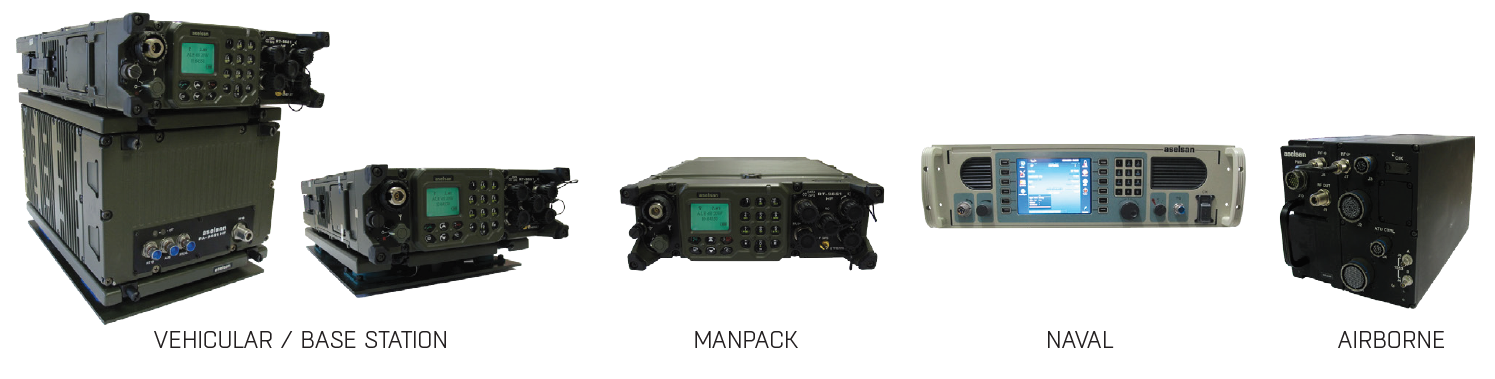
\includegraphics[width=1.0\unitlength]{radio_type}
	\caption{\label{fig:radtyp}ASELSAN 9661 Radio Series }
\end{figure}

	The radio has embedded Built-In Digital Modem. Modem functionalities in the Software Defined HF Radio are implemented based on several NATO STANAGs and MIL-STD's. While voice and data can be transmitted over a preset fixed frequency, it is also possible to employ an Automatic Channel Selection mechanism which determines the usable frequency for communication. It is possible to communicate under intentional or unintentional interference by using frequency hopping mode of operation.

	9661 HF Radio built-in modem (physical layer) includes Digital Data Waveforms, Automatic Link Establishment and Frequency Hopping. USB, LSB, ISB, AME, AM and CW modulations are supported through 9661 HF Software Defined Radio.  

\begin{figure}[H]
	\center
	\setlength{\unitlength}{\textwidth} 
	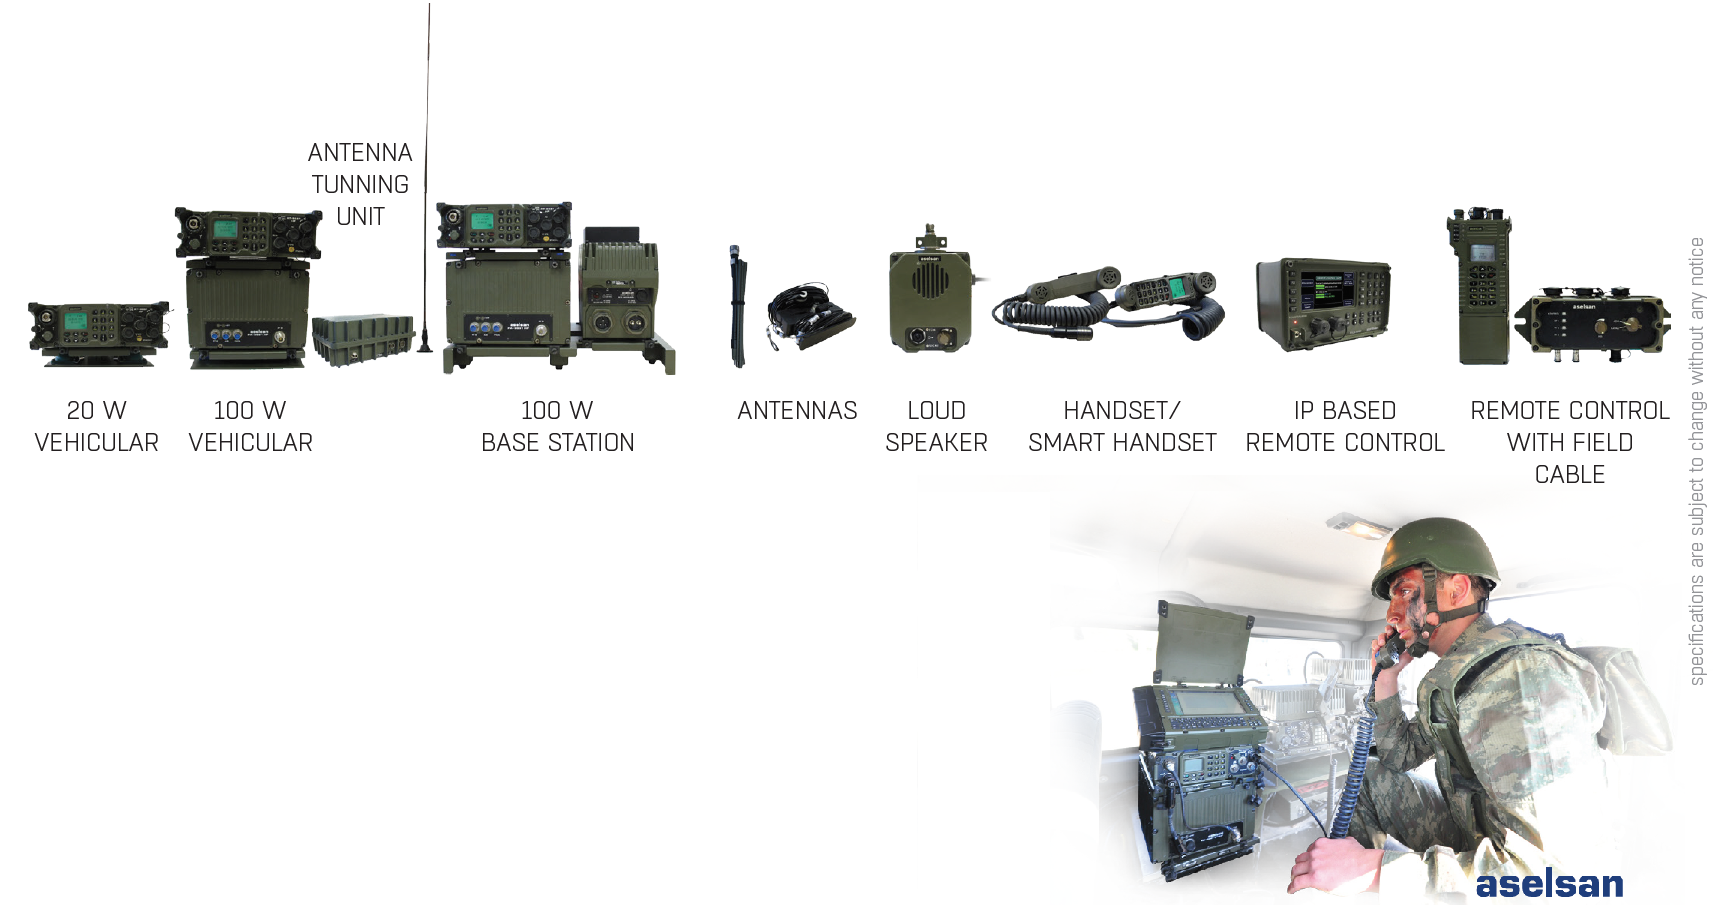
\includegraphics[width=1.0\unitlength]{radios}
	\caption{\label{fig:rads}ASELSAN 9661 Radio Series }
\end{figure}

	Digital voice coding/decoding is performed with MELPe vocoder and the data rate for digital voice can be 600, 1200 or 2400 bps. Digital voice communication over fixed frequency can be encrypted. Data communication over fixed frequency can be encrypted or clear. Frequency hopping is the Electronic Protection Measure (EPM) for transmission of digital voice and data.

	9661 HF Radio family has three configurations for Manpack, Vehicle and Fixed Station usage. 20W can be used for Manpack and Vehicle configurations and 150 W can be used for Vehicle and Fixed Station configurations.

\vfill

\begin{figure}[H]
	\center
	\setlength{\unitlength}{\textwidth} 
	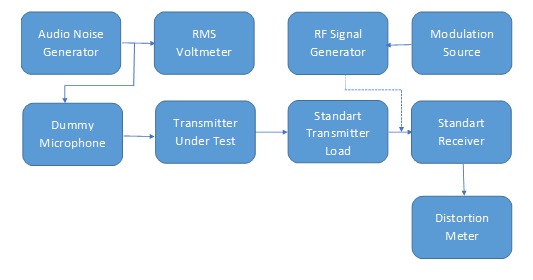
\includegraphics[width=1.0\unitlength]{elecaudio}
	\caption{\label{fig:elecaudio}ASELSAN 9661 Radio Series }
\end{figure}




\begin{figure}[H]
	\center
	\setlength{\unitlength}{\textwidth} 
	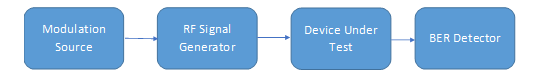
\includegraphics[width=1.0\unitlength]{refsens}
	\caption{\label{fig:refsens}ASELSAN 9661 Radio Series }
\end{figure}


\begin{figure}[H]
	\center
	\setlength{\unitlength}{\textwidth} 
	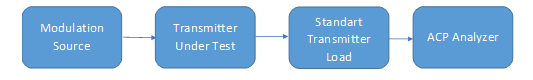
\includegraphics[width=1.0\unitlength]{transnoise}
	\caption{\label{fig:transnoise}ASELSAN 9661 Radio Series }
\end{figure}

\begin{figure}[H]
	\center
	\setlength{\unitlength}{\textwidth} 
	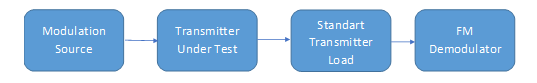
\includegraphics[width=1.0\unitlength]{c4fmmod}
	\caption{\label{fig:c4fmmod}ASELSAN 9661 Radio Series }
\end{figure}

\subsubsection{Modulation Fidelity Test}
\- \indent

	Modulation fidelity is the degree of closeness to which the modulation follows the desired ideal therotical modulation.The fidelity is determined by from observations of the signal at the output of an integrate and dump filter, that is preceded by an FM demodulator. The filtered FM modulation trajectories for C4FM and CQPSK are different at all points in time except at the symbol decision points.
	
	The modulation fidelity is measured by determining the rms difference between the actual signal and the ideal C4FM deviation for the transmitted symbols as information.
	
\begin{table}[H]
  \centering
 
    \begin{tabular}{c|c|c}
       $$Bits$$ & $$Symbols$$ & $$C4FM Deviation$$ \\ \hline
       00 & +3 & +1.8 kHz  \\ \hline
       01 & +1 & +0.6 kHz  \\ \hline
       10 & -1 & -0.6 kHz  \\ \hline
       11 & -3 & -1.8 kHz  
      
  \end{tabular}
  \caption{modfide}
  \label{tab:modfide}
\end{table}

	Let $s_K$ represents the C4FM deviation of the transmitted symbols, and $z_K$ represents the detected signals at $t_K$ sampling instants.
	
	The transmitter can be modelled as
	
	$$ z_K~=~C_O+C_L*(s_K~+~e_K) $$
	
	where $C_O$ is a constant representing carrier frequency offset and the $C_L$ is another constant called deviation errors that is resulting from gain errors in the transmitter's modulator baseband signal processing. And $e_K$ is called residual deviation error.
	
	
\begin{figure}[H]
	\center
	\setlength{\unitlength}{\textwidth} 
	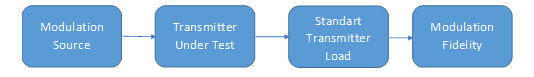
\includegraphics[width=1.0\unitlength]{modfide}
	\caption{\label{fig:modfide}ASELSAN 9661 Radio Series }
\end{figure}






\subsection{Tests on ULAK 4.5G Base Station  }

\subsubsection{ULAK 4.5G Macrocell Base Station}
\- \indent
	Based on Release 10 and Release 11 standards published by 3GPP, ULAK Macrocell Base Station is designed to support both Release 12 and Release 13 standards with flexible architecture that is open to software development without any hardware changes and is designed to work on different frequency bands for use in Commercial or Public Safety networks.  

\begin{figure}[H]
	\center
	\setlength{\unitlength}{\textwidth} 
	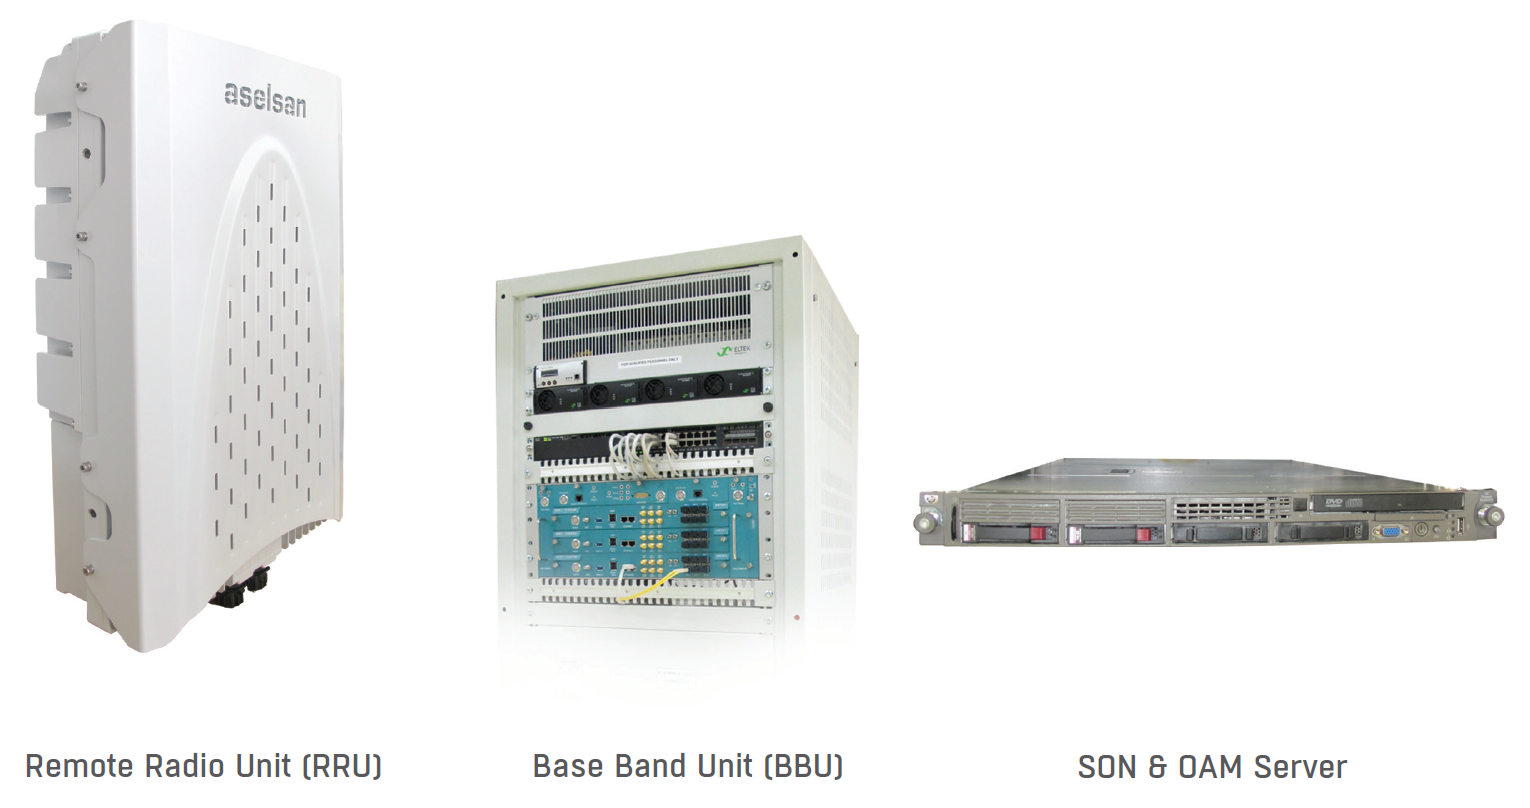
\includegraphics[width=1.0\unitlength]{ulak}
	\caption{\label{fig:ulak}ULAK 4.5G Base Station }
\end{figure}	
	
	To enrich the product portfolio; the following studies are currently carried out:

	Integration of LTE-A to Narrowband Communication Systems,
LTE-Advanced Mobile Terminal Safety Software  
With the development of 4.5G Communication Systems, it is aimed to meet the need of fast, secure and continuous communication of both mobile operators and public institutions.


\vfill


\subsection{Outer Space Simulations \& Tests using TVAC  }

\subsubsection{Thermal Vacuum Chamber (TVAC) }

	A vacuum chamber is a rigid enclosure from which air and other gases are removed by a vacuum pump. This results in a low-pressure environment within the chamber, commonly referred to as a vacuum. A vacuum environment allows researchers to conduct physical experiments or to test mechanical devices which must operate in outer space (for example) or for processes such as vacuum drying or vacuum coating. Chambers are typically made of metals which may or may not shield applied external magnetic fields depending on wall thickness, frequency, resistivity, and permeability of the material used. Only some materials are suitable for vacuum use.

Chambers often have multiple ports, covered with vacuum flanges, to allow instruments or windows to be installed in the walls of the chamber. In low to medium-vacuum applications, these are sealed with elastomer o-rings. In higher vacuum applications, the flanges have knife edges machined onto them, which cut into a copper gasket when the flange is bolted on.

\begin{figure}[H]
	\center
	\setlength{\unitlength}{\textwidth} 
	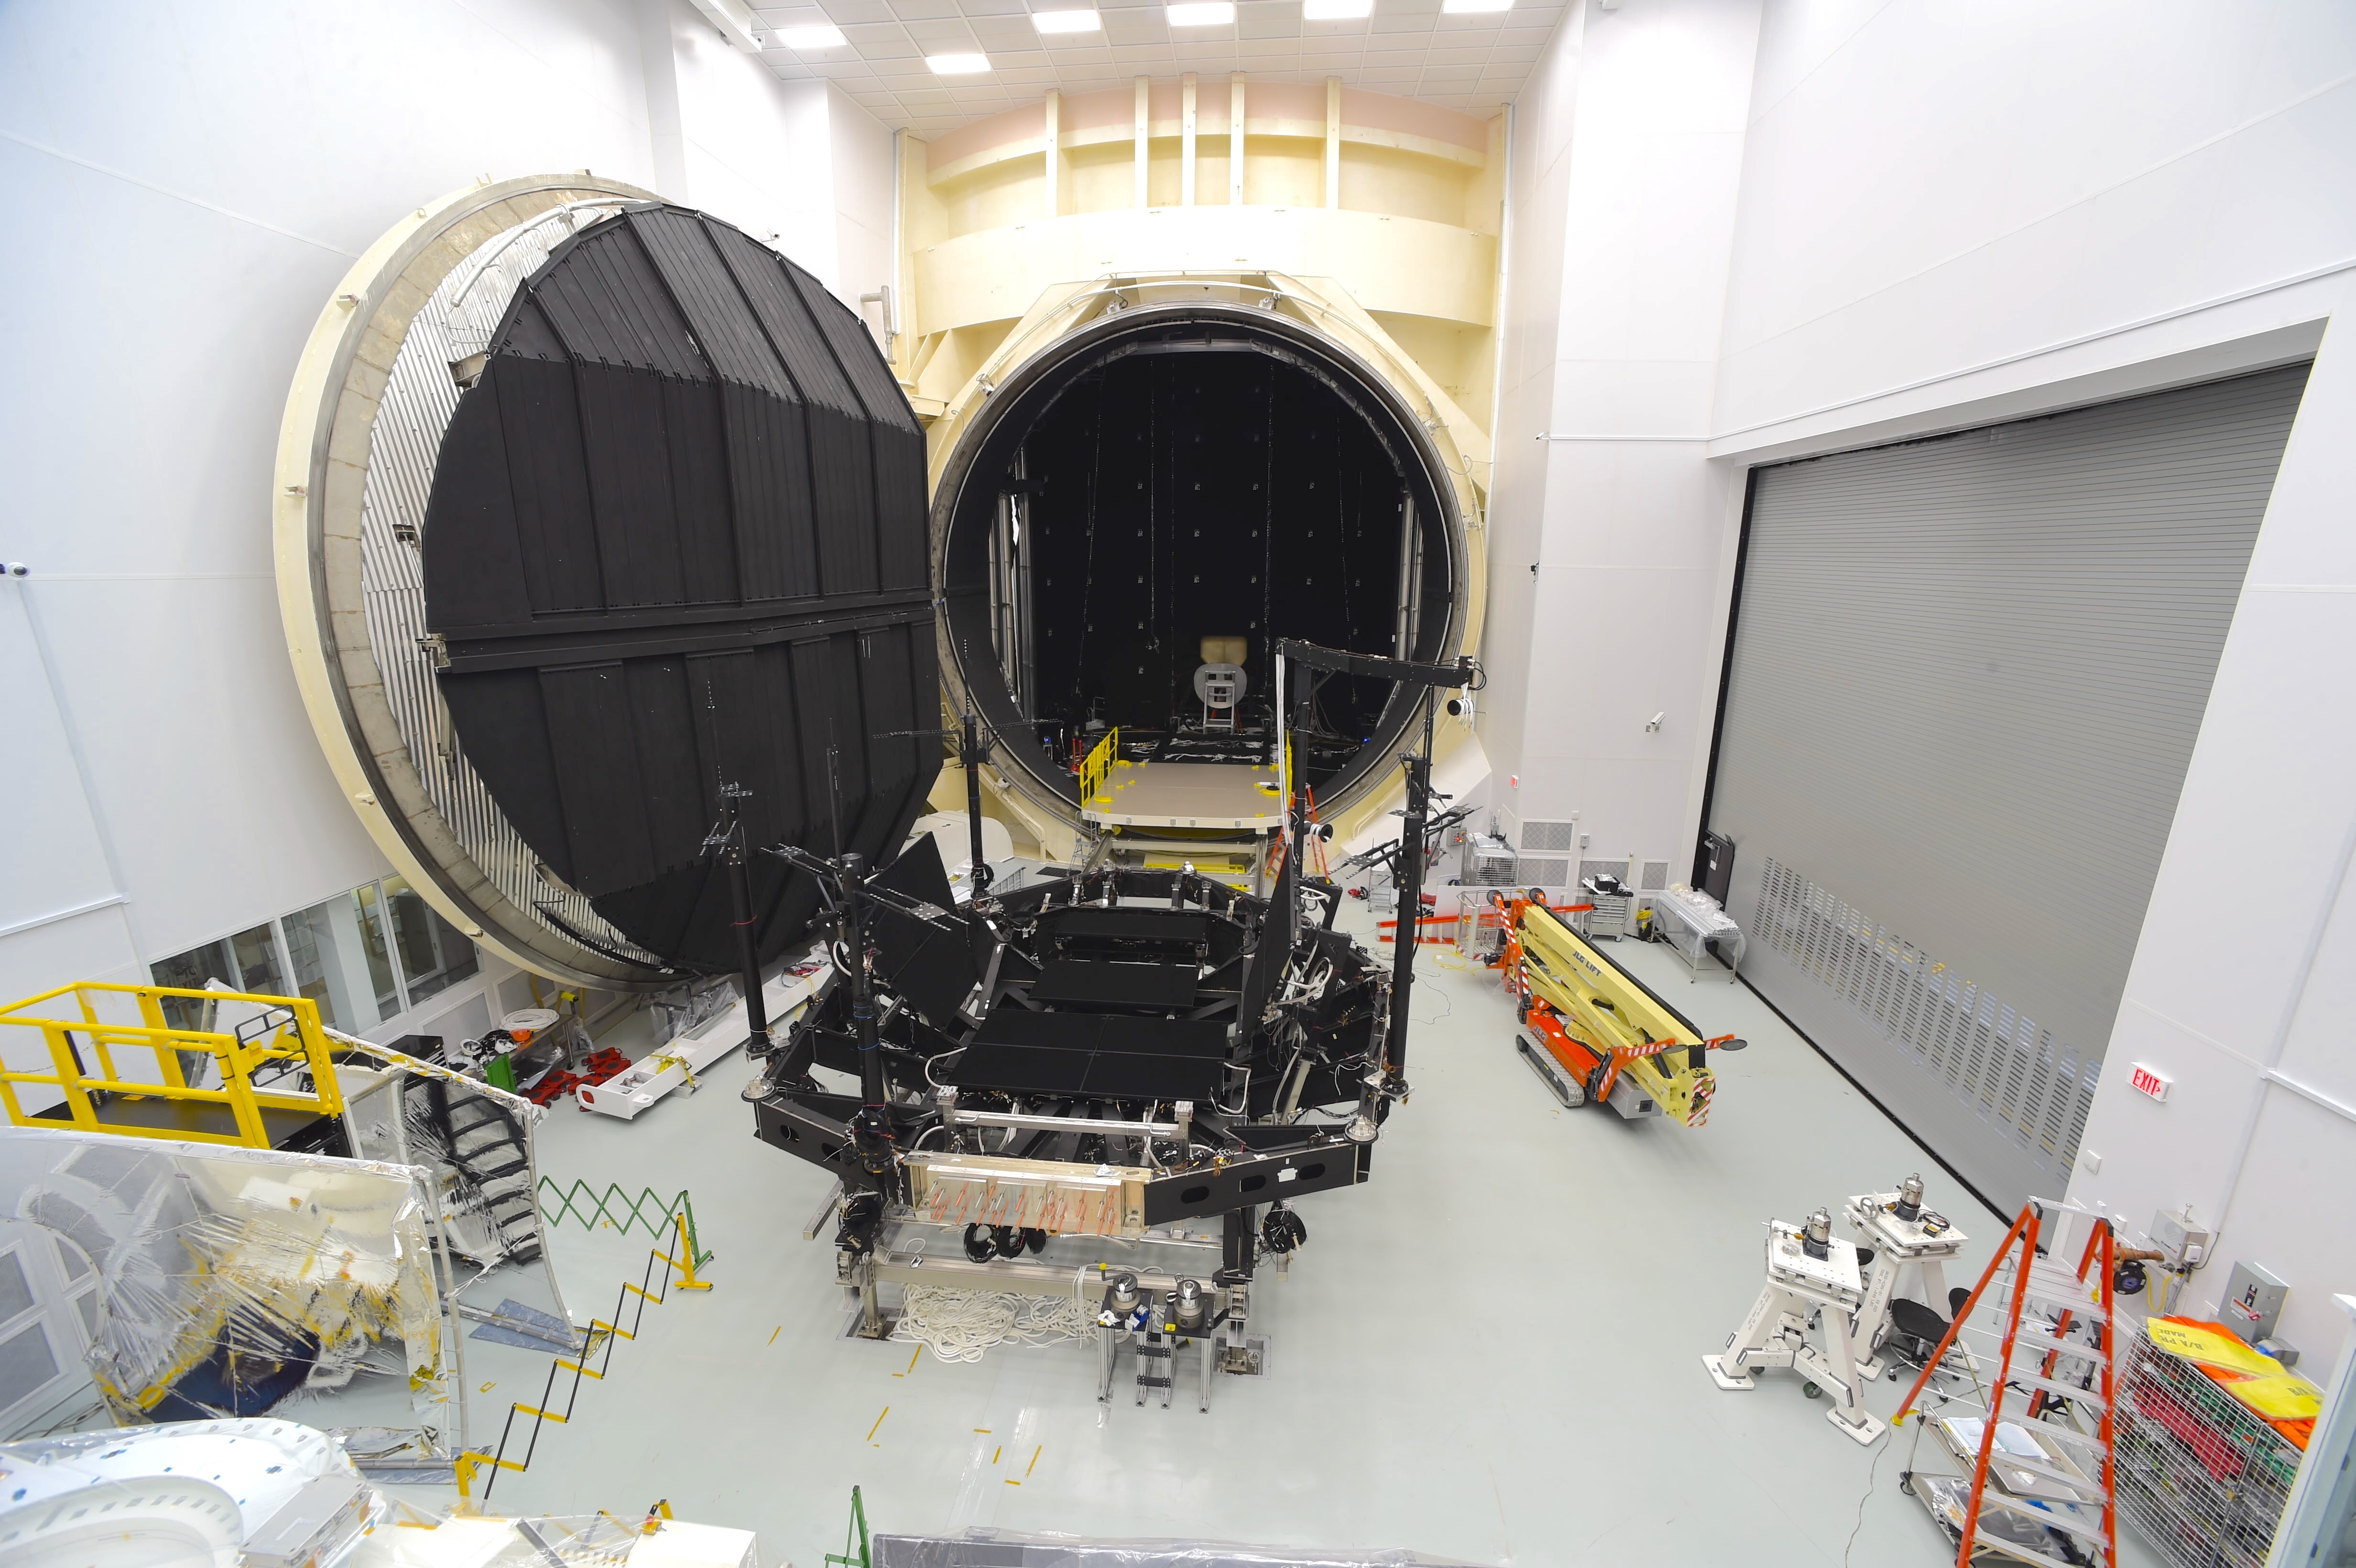
\includegraphics[width=1.0\unitlength]{tvac}
	\caption{\label{fig:tvac}An Example Thermal Vacuum Chamber }
\end{figure}

A type of vacuum chamber frequently used in the field of spacecraft engineering is a thermal vacuum chamber, which provides a thermal environment representing what a spacecraft would experience in space.

	A thermal vacuum chamber is a vacuum chamber in which the radiative thermal environment is controlled.

Typically the thermal environment is achieved by passing liquids or fluids through thermal shrouds for cold temperatures or through the application of thermal lamps for high temperatures.

Thermal vacuum chambers are frequently used for testing spacecraft or parts thereof under a simulated space environment.

\subsection{Research on Components of ULAK 4.5G Base Station  }

\subsubsection{Alternate Components}

\- \vfill
%\begin{enumerate}
%\item --
%\item --
%\item --
%\item --
%\item --
%\item --
%\end{enumerate}

%\begin{figure}[H]
%\centering
%%<\includegraphics[scale=1.0]{todo2.jpg}
%\caption{\label{fig:------} ------ ------  }
%\end{figure}
								
	
%\begin{table}[H]
%  \centering
 
%    \begin{tabular}{c|c|c}
%       &$$------$$ & $$------------$$ \\ \hline
%       1 & -- & ---  \\ \hline
%       2 & -- & ---  \\ \hline
%       3 & -- & ---  \\ \hline
%       4 & -- & ---  \\ \hline
%       5 & -- & ---  \\ \hline
%       6 & -- & --- 
%      
%  \end{tabular}
%  \caption{------}
%  \label{tab:------}
%\end{table}
	
	
%\begin{lstlisting}[style=CStyle]


%----


%\end{lstlisting}

%\vfill

%\begin{lstlisting}[language=Matlab]

%----

%\end{lstlisting}



\section{Conclusion}

\-
\indent I completed my summer practice in ASELSAN A.Ş.(ASELSAN Electronics Industry and Ticaret A.Ş.) in supervision of Pınar Kırıkkanat, an electronics engineer in ASELSAN, in Yenimahalle/Ankara. It was quite experiential time for me. Throughout my summer practice, I learned many things about professional work life. 

	Firstly, I understodd the importance of mandatory educations like occupational safety and health education thanks to given educations by ASELSAN. After the educations, I was  sent to my division, where I performed my summer practice.
	
	In the first half of my internship, I was given time to observe, learn and participate the mechanical and electrical test conducted at our division. Mainly on ASELSAN 9661 Series Radios, I mostly observed and participated on the environmental tests of the equipments produced at the Communication \& Information Technologies Vice Presidency, known as HBT. .
	
	In the second part of my internship, I was given time to observe the work done behind the testing, in other words process design and management. In this part of my internship, I participated on documentation and research activities for the ULAK Base station of the ASELSAN. Since the work done at this stage can be mostly considered as classified information, I will mention the basics of what I have done in this part.
	
	In this, report, I start with an introduction, that covers what was done in my summer practice. Then, I continued with a company description section in which the general description about ASELSAN is given. After that part, the work done in my summer practice is explained. Lastly, I finished the report with an conclusion part. 
		
	
	Finally, I recommend my summer practice company for other students who want to start their summer practice at ASELSAN. 

\-\vfill 


\section{References}

\begingroup
\renewcommand{\section}[2]{}%
%\renewcommand{\chapter}[2]{}% for other classes
\begin{thebibliography}{}

\bibitem{gitsun} Temurtas Halil,
	\textit{Sun Tracker System},
	Bitbucket repository,(2017),
	https://bitbucket.org/temurtas/pi/
	
\bibitem{defense}	A,	
https://people.defensenews.com/top-100/	
	
\bibitem{attinf}	A,
	https://www.radio-electronics.com/info/rf-technology-design/attenuators/rf-attenuators-basics-tutorial.php

\bibitem{attpic}	B,
	https://nelsoncreated.com/products/attenuators-2/ 

\bibitem{powref}	C,
	http://www.livingston-products.com/products/pdf/105517\_1\_en.pdf

\bibitem{audany}	D,
	https://www.rohde-schwarz.com/us/brochure-datasheet/upv/

\bibitem{tvac}	E,
	https://www.nasa.gov/feature/goddard/2017/nasas-apollo-era-test-chamber-now-james-webb-space-telescope-ready

\bibitem{diss}	F,
https://www.csgb.gov.tr/media/4574/kitap01.pdf

\end{thebibliography}
\endgroup

\vfill


\appendix








\tikzset{
desicion/.style={
    diamond,
    draw,
    text width=4em,
    text badly centered,
    inner sep=0pt
},
block/.style={
    rectangle,
    draw,
    text width=10em,
    text centered,
    rounded corners
},
cloud/.style={
    draw,
    ellipse,
    minimum height=2em
},
descr/.style={
    fill=white,
    inner sep=2.5pt
},
connector/.style={
    -latex,
    font=\scriptsize
},
rectangle connector/.style={
    connector,
    to path={(\tikztostart) -- ++(#1,0pt) \tikztonodes |- (\tikztotarget) },
    pos=0.5
},
rectangle connector/.default=-2cm,
straight connector/.style={
    connector,
    to path=--(\tikztotarget) \tikztonodes
}
}

\tikzset{
desicion/.style={
    diamond,
    draw,
    text width=4em,
    text badly centered,
    inner sep=0pt
},
block/.style={
    rectangle,
    draw,
    text width=10em,
    text centered,
    rounded corners
},
cloud/.style={
    draw,
    ellipse,
    minimum height=2em
},
descr/.style={
    fill=white,
    inner sep=2.5pt
},
connector/.style={
    -latex,
    font=\scriptsize
},
rectangle connector/.style={
    connector,
    to path={(\tikztostart) -- ++(#1,0pt) \tikztonodes |- (\tikztotarget) },
    pos=0.5
},
rectangle connector/.default=-2cm,
straight connector/.style={
    connector,
    to path=--(\tikztotarget) \tikztonodes
}
}

\vfill % Fill the rest of the page with whitespace
\end{document}